\documentclass[0-protokol.tex]{subfiles}
\begin{document}

Torzní magnetometr je sestaven zavěšením magnetického dipólu - v praxi stálého magnetu - na kovovém vlákně. V této úloze měříme úhel vychýlení dipólu působením vnějších magnetických sil, proto závěs opatříme zrcátkem, které promítá laserový paprsek na číselnou stupnici. Vnější magnetické pole realizujeme upevněním kruhové cívky tak, aby její osa směřovala kolmo na kovové vlákno a zavěšený dipól se nacházel co možná nejblíže středu cívky. Pro měření využijeme zapojení \ref{fig:zapojeni} \cite{stud_text}.

Z důsledku Biotova-Savartova zákona platí pro intenzitu magnetického pole kruhové cívky o poloměru $r$ a počtu závitů $N$ protékané proudem $I$ vztah 
\begin{equation} \label{eq:H_civky}
H = \frac{NI}{2r}.
\end{equation}

Pro intenzitu magnetického pole zároveň platí 
\begin{equation} \label{eq:H_vychylka}
H = \frac{\alpha D}{p},
\end{equation}
kde $p$ jeho Coulombův magnetický moment a $D$ direkční moment vlákna.

Rovnovážnou výchylku zavěšeného magnetu $\alpha$ spočítáme ze vzdálenosti zrcátka od stupnice $l$ a posunutí světelné značky na stupnici $x$ jako
\begin{equation} \label{eq:alpha}
\alpha \approx \frac{x}{2L}.
\end{equation}
Tento vztah je přibližný, pro hodnoty měřené v tomto praktiku však dostatečný.

\begin{figure}[H]
\centering
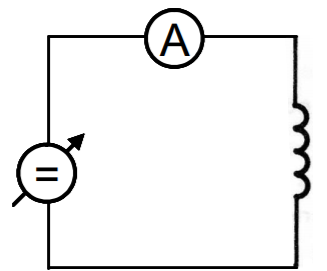
\includegraphics[scale=0.7]{zapojeni}
\caption{Zapojení pro měření torzním magnetometrem}
\label{fig:zapojeni}
\end{figure}

Kombinací uvedených vztahů dostaneme rovnici, kterou použijeme pro ověření Biotova-Savartova zákona,
\begin{equation} \label{eq:B-S}
I = \frac{2rD\alpha}{Np}.
\end{equation}

Pro určení magnetického momentu zavěšeného magnetu určíme direkční moment kovového vlákna metodou torzních kmitů pomocí vztahu 
\begin{equation} \label{eq:D}
D = \frac{4\pi^2 J}{T^2},
\end{equation}
kde $J$ je známý moment setrvačnosti kovové tyčky, kterou pro tento účel upevníme na závěs, a $T$ je perioda kmitů.

Pro výpočet Coulombova magnetického momentu zavěšeného magnetu použijeme směrnici\,$S$ lineární regrese závislosti výchylky magnetometru na proudu protékajícím cívkou. Ze vztahu\,\ref{eq:B-S} odvodíme
\begin{equation} \label{eq:p}
p = \frac{2 r D S}{N}.
\end{equation}
Ampérův magnetický moment pak spočteme jako 
\begin{equation} \label{eq:m}
m = \frac{p}{\mu_0},
\end{equation}
kde $\mu_0 = \SI{4\pi e-7}{\henry\per\metre}$ je permeabilita vakua.

\subsection*{Statistické vyhodnocení}
Průměrná hodnota naměřených veličin při $n$ měřeních je počítána podle vzorce aritmetického průměru 
\begin{equation}
\overline{x} = \frac{1}{n} \sum\limits_{i=1}^n{x_i}.
\end{equation}
Statistická chyba $\sigma_{stat}$ aritmetického průměru se získá ze vztahu 
\begin{equation}
\sigma_{stat} = \frac{\sqrt{\frac{1}{n-1} \sum\limits_{i=1}^n{(x_i - \overline{x})^2}}}{\sqrt{n}}.
\end{equation}
Absolutní chyba je potom získána z $\sigma_{stat}$ a chyby měřidla $\sigma_{\textit{měř}}$ jako 
\begin{equation}
\sigma = \sqrt{\sigma_{\textit{měř}}^2 + \sigma_{stat}^2}.
\end{equation}

Chyba výpočtů se řídí zákonem přenosu chyb.

\end{document}

